\chapter[Klassifikation Homomorpher Kryptosysteme]{\texorpdfstring{Klassifikation Homomorpher\\ Kryptosysteme}{Klassifikation Homomorpher Kryptosysteme}}
\label{KHK}

In diesem Kapitel werden verschiedene Anwendungen vorgestellt, in denen ein oder mehrere semihomomorphe Kryptosysteme zum Einsatz kommen. 

Für eine Klassifizierung erfolgt die Untersuchung der Anwendungen unter folgenden Kriterien:
\begin{enumerate}
	\item Es sollen die \textit{Eigenschaften eines semihomomorphen Kryptosystems identifiziert} werden, welches Wissenschaftler zu deren Einsatz bewegt hat.
	\item Es wird untersucht, welche \textit{Funktionen und Operatoren} mit der homomorphen Verknüpfung eines Kryptosystems realisiert werden.
	\item Die verwendeten Kryptosysteme können nur IND-CPA oder IND-CCA1 sicher sein. Sie sind insbesondere nicht NM-sicher. Es wird ausgeführt, inwiefern dies bei der Implementierung berücksichtigt wird, um die \textit{Integrität} von Rechenoperationen zu gewährleisten.
\end{enumerate} 

\section{Autocrypt \cite{tople2013autocrypt}}
\label{autocrypt}
Server sind ständig durch Angriffe bedroht, die bis hin zu ihrer kompletten Übernahme führen können. Um Datendiebstahl und Vertraulichkeitsverletzungen vorzubeugen, ist es ratsam nur mit verschlüsselten Datenbeständen auf den Servern zu arbeiten. Die Anpassung der Programme, um mit verschlüsselten Daten zu arbeiten, wollen die Wissenschaftler automatisieren, indem sie die Arbeit der Programmtransformation mit einem selbst entwickelten Compiler abwickeln. Das Ergebnis ihrer Forschung ist der Compiler Autocrypt.

Ein Server läuft als nicht vertrauenswürdige virtuelle Maschine (VM). Inhalte werden außerhalb der VM auf einem vertrauenswürdigen Schlüsselserver verschlüsselt. Autocrypt bestimmt automatisch welche Verschlüsselung des Wertes einer Variable für Rechenoperationen notwendig sind und konvertiert ihren Wert im Programmablauf durch Einfügen von Hypercalls\footnote{Ein Hypercall ist vergleichbar mit einem Systemaufruf in der Virtualisierungsumgebung. Ein Hypercall ermöglicht die Ausführung von Instruktionen die höhere Rechte benötigen. https://wiki.xenproject.org/wiki/Hypercall}. In Abhängigkeit davon, welche mathematische Grundoperation mit einer Variable ausgeführt wird, rechnet das transformierte Programm mit der passenden Darstellung im semihomomorphen Kryptosystem. Wenn im Ursprungscode Additionen von zwei Variablen durchgeführt werden, werden ihre Wert mit Paillier\footnote{Paillier ist ein additiv semihomomorphes Kryptosystem \cite{paillier1999public}.} verschlüsselt. Wird das Ergebnis allerdings später multipliziert, dann muss der Wert einer Variable zur Laufzeit konvertiert werden nach ElGamal\footnote{ElGamal ist ein multiplikativ semihomomorphes Kryptosystem \cite[p.32]{yi2014homomorphic}.}. Veranschaulicht wird dies in Abbildung \ref{fig:autocrypt}. Durch die Konvertierung der Werte zwischen Darstellungen in Paillier und ElGamal wird die Verwendung eines langsameren vollhomomorphen Kryptosystems vermieden.

\begin{figure}[h]
	\begin{center}
		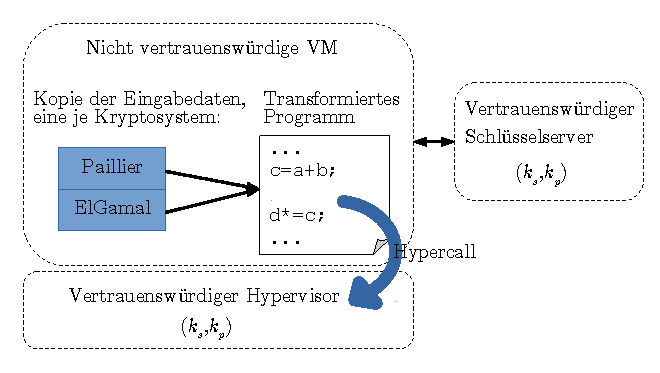
\includegraphics{fig/Autocrypt}
		\caption{Die nicht vertrauenswürdige VM führt an einer Stelle im Programm einen Hypercallaufruf aus, um den Wert in der Variable c von Paillier nach ElGamal zu konvertieren. Alle Eingabedaten des Programms liegen in der VM verschlüsselt vor. Die Konvertierung wird von dem vertrauenswürdigen Hypervisor ausgeführt. }
		\label{fig:autocrypt}
	\end{center}
\end{figure}

Bei der Entwicklung von Autocrypt ist das primäre Ziel alle Rechenoperationen unter Wahrung der Privatsphäre durchzuführen. Die Forscher erwähnen explizit, dass es nicht Ziel ist die Integrität der verarbeiteten Daten eines transformierten Programms sicherzustellen.

\textbf{Zur Sicherheit des transformierten Programms:}
Es wird angenommen, dass die zu transformierenden Programme keine Größen von verarbeitenden Daten verbergen müssen. Man geht davon aus, dass im zu transformierenden Programm Maßnahmen gegen Seitenkanalangriffe umgesetzt worden. Es wird jedoch nicht darauf eingegangen, inwiefern dieser Schutz unter der Transformation durch Autocrypt erhalten bleibt. Die semantische Sicherheit von Paillier und ElGamal wird genutzt, um eine Sicherheit gegenüber dem IND-CPA Angreifermodell für alle Operationen auf der VM garantieren. Hierzu skizzieren die Autoren einen Beweis.

Autocrypt realisiert homomorphe Operation auf Bits durch Verwendung des Paillier Kryptosystems für die Bitdarstellung von Integern anstelle des Integerwerts selbst. Wie Autocrypt mit Fließkommazahlen umgeht wird nicht erwähnt.

\textbf{Klassifizierungskriterien:}
\begin{enumerate}
	\item Die semantische Sicherheit der semihomomorphen Kryptosysteme von Paillier und ElGamal ist Grundlage um von Autocrypt transformierte Programme sicher gegenüber IND-CPA Angreifern zu machen. Es wird eine Kombination aus additiven und multiplikativen semihomomorphen Kryptosystemen für Rechenoperationen im transformierten Programm verwendet, da diese effizienter sind als untersuchte vollhomomorphe Kryptosysteme. 
	\item Das Paillier Kryptosystem wird eingesetzt, um homomorphe Bitoperationen zu ermöglichen.
	\item Eine Integrität der Rechenoperationen wird ausdrücklich nicht berücksichtigt.
\end{enumerate}

\section[Machine Learning Classification over encrypted data  \cite{bost2015machine}]{\texorpdfstring{Machine Learning Classification over encrypted data\\  \cite{bost2015machine}}{Machine Learning Classification over encrypted data  \cite{bost2015machine}}}
\label{ML}
Es wird ein Privatsphäre wahrendes\footnote{privacy-preserving, siehe: \ref{privacypreserving}} Verfahren des Maschienenlernens entworfen, bei dem sowohl die zu klassifizierenden Daten (zusammengefasst in Merkmalsvektoren\footnote{Ein Merkmalsvektor ist eine einheitliche Darstellung des zu klassifizierenden Objektes. }) als auch die Klassifizierermodelle\footnote{Der Klassifizierer C benutzt das Klassifizierermodell w um den Merkmalsvektor x einer Klasse c=C(x,w) zuzuordnen.} vertraulich bleiben. Dazu wird eine Bibliothek konstruiert, aus der modular beliebige Privatsphäre wahrende Klassifizierer erstellt werden können.

\begin{figure}[h]
	\begin{center}
		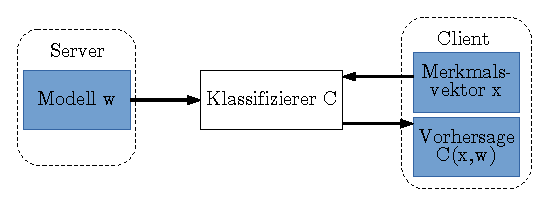
\includegraphics{fig/ML}
		\caption{Der nicht vertrauenswürdige Klassifizierer enthält verschlüsselte Eingaben vom Server und Client. Nach der Klassifizierung darf der Server nichts über die Merkmalsvektoren vom Clienten und der Client darf nichts über das Modell für die Klassifizierung vom Server lernen.}
		\label{fig:ML}
	\end{center}
\end{figure}

In dem Design dieser Module werden homomorphe Kryptosysteme verschieden eingesetzt:

Für die Klassifizierung müssen die Module Vergleichsoperationen $(<,\leq)$ zwischen verschlüsselten Werten durchführen können. Die Autoren verwenden hierzu ein Protokoll von Veugen \cite{veugen2011comparing}, dass mit jedem semantisch sicheren homomorphen Kryptosystem verwendet werden kann. Veugen selbst evaluiert die Performance des Protokolls unter Verwendung der Kryptosysteme von Goldwasser-Micali\footnote{Das Kryptosystem von Goldwasser-Micali erlaubt eine homomorphe bitweise XOR Verknüpfung. \cite{goldwasser1984probabilistic}} und Paillier. Da die Autoren dieser Studie keine weiteren Gründe für den Einsatz gerade dieser Kryptosysteme aufführen, wird angenommen, dass sie sich an dem Beispiel von Veugen orientieren.

Weiter sollen die Klassifizierer Polynome evaluieren können, die einen binären Entscheidungsbaum repräsentieren (siehe Abbildung \ref{fig:Baum}): Die Blätter des Entscheidungsbaums sind mögliche Klassen $c$, zu denen der Merkmalsvektor $x$ zugeordnet werden kann. Den Weg im Entscheidungsbaum zu gehen, entspricht der privaten Evaluation des Polynoms, dass diesen Entscheidungsbaum repräsentiert. Für die Evaluation des Entscheidungsbaums geben die Autoren eine Tiefe von $\text{log}_2\cdot h_{max}$ Multiplikationen an. Durch diese beschränke Tiefe von Rechenoperationen eignet sich der der Einsatz des eingeschränkten (hier: leveled) vollhomomorphen Kryptosystems von Brakerski-Gentry-Vaikuntanathan\footnote{Die Autoren verwenden HELib, eine Bibliothek die das Kryptosystem von Brakerski-Gentry-Vaikuntanathan implementiert.} (BGV). Das BGV Kryptosystem ist IND-CPA sicher \cite{Brakerski2012LeveledFH}.
%Verschlüsselung der Eingabeparameter in Binärdarstellung für noch mehr Performance

\begin{figure}[h] 
	\begin{center}
		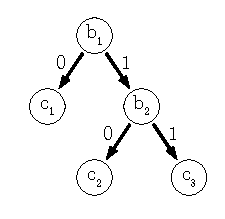
\includegraphics{fig/Baum}
		\caption{Damit der Klassifizierer in einem binärem Baum privat einen Pfad von der Wurzel zum Blatt geht, wird dieser als ein Polynom repräsentiert, das privat berechnet wird. Der Wert des Knotens $b_i\in\{0,1\}$ bestimmt, welchen Pfad entlang gegangen wird und ist von einem Vergleich aus Einträgen des Modells $w$ und Merkmalsvektors $x$ abhängig. z.B. Falls $x_1\leq w_1 \rightarrow b_1=1$. Das zu diesem Baum zugehörige Polynom ist: $P(b_1,b_2,c_1,c_2,c_3)=b_1(b_2\cdot c_3+(1-b_1)c_2)+(1-b_1)c_2$.}
		\label{fig:Baum}
	\end{center}
\end{figure}
% Das Polynom evaluiert zu c iff x...

Als Vorteil des Einsatzes von Paillier wird ein großer Klartextraum von $2^{1024}$ Bit genannt. Die Größe des Klartextraums wird genutzt, um Fließkommazahlen zu verschlüsseln, indem diese durch Multiplikation mit großen Exponenten zu Integern konvertiert werden.

Ein weiterer Einsatz von Paillier erfolgt in der Berechnung eines privaten Skalarproduktes zwischen zwei Parteien:

Gegeben seien die Vektoren $x=(x_1,\ldots,x_n)$ von A und $y=(y_1,\ldots,y_n)$ von B, wobei alle Einträge Klartexte sind. Sei $k=(k_s,k_p)$ das Schlüsselpaar im Paillier-Kryptosystem:

\begin{enumerate}
	\item B verschlüsselt die Komponenten $y_i$ mit $k_s$ und sendet $e_{k_s}(y_i)$ an A.
	\item A berechnet $x_i\cdot y_i$ durch Potenzierung des Chiffretextes von B mit $x_i$. Dies funktioniert genauso wie im Okamoto-Uchiyama Kryptosystem in Abschnitt \ref{OUK}. Unterschied ist lediglich der Modulus\footnote{Bei Okamoto-Uchiyama ist der Modulus $n=p^2 q$. In beiden Fällen sind $p,q$ Primzahlen.}  von $n^2$  bei Paillier mit $n=pq$. Durch Multiplikation der Chiffretexte wird dann die i-te Komponente im Klartext aufsummiert:	
	\begin{equation*}
		e_{k_s}(\left\langle x,y\right\rangle )=\prod_i e_{k_s}(y_i)^{x_i} \text{ mod } n^2.
	\end{equation*}
\end{enumerate}

\textbf{Klassifizierungskriterien:}
\begin{enumerate}
	\item Die semihomomorphen Kryptosysteme von Goldwasser-Micali und Paillier werden verwendet, um verschlüsselte Werte bzgl. ihrer numerischen Größe zu vergleichen. Der große Klartextraum von Paillier wird genutzt, um Fließkommazahlen zu verschlüsseln. Das beschränkte vollhomomorphe Kryptosystem von Brakerski-Gentry-Vaikuntanathan wird eingesetzt, um Polynome zu evaluieren.
	\item Es wird ein privates Skalarprodukt auf Basis von Paillier implementiert.
	\item Der Einsatz von homomorphen Kryptosystemen geschieht nur unter dem Hintergrund die Daten vertraulich zu verarbeiten. Es wird weder die Möglichkeit einer unautorisierten Verformbarkeit ausdrücklich erwähnt, noch in dem Design der Module zur Konstruktion von Klassifizierern berücksichtigt. Die Autoren gehen jedoch von einem honest-but-curious Angreifermodell aus, d.h. es wird angenommen, dass ein Angreifer jegliche Kommunikation mitlesen kann, sich jedoch protokollkonform verhält. Insbesondere kann er nicht die Verschlüsselung brechen. Da die Eingabedaten des Klassifizierers verschlüsselt sind, kann der Angreifer keine Einsicht in ihre Inhalte bekommen.
	\end{enumerate}

\section{Privacy Preserving Matrix Factorization \cite{nikolaenko2013privacy}}
\label{PPMF}
Für die Generierung von personenspezifischen Empfehlungen wird Matrixfaktorisierung verwendet \cite{koren2009matrix}. Die Matrixfaktorisierung ist Bestandteil eines Empfehlungssystems (engl. \textit{recommender system}), das anhand vorheriger Bewertungen die Personen für Objekte abgegeben haben, zukünftige Empfehlungen geben kann (z.B. Einkäufe in einem Onlineladen).

In dieser Studie möchten die Wissenschaftler ein Empfehlungssystem entwerfen, dass die Matrizenfaktorisierung unter Wahrung der Privatsphäre der abgegebenen Bewertungen durchführt. Das Empfehlungssystem soll Empfehlungen geben können ohne die abgegebenen Bewertungen einer Personen zu lernen oder die Objekte welche Personen bewertet haben. Es werden nur die Objektkategorien  gelernt.

Die Matrixfaktorisierung wird von dem Empfehlungssystem in Kooperation mit einem Schaltkreisanbieter durch Anwendung des \enquote{Garbled Circuit} Protokolls von Yao \cite{yao1982protocols} durchgeführt (siehe Abbildung \ref{fig:Matrix}). Es wird nun die Kommunikation zwischen Empfehlungssystem und Schaltkreisanbieter erläutert: Das Empfehlungssystem erhält mit Hash-ElGamal\footnote{Hash-ElGamal ist ein semihomomorphes Kryptosystem zur XOR Verknüpfung \cite[Appendix B]{nikolaenko2013privacy} und IND-CPA sicher \cite[p.6]{chevallier2006encoding}.} verschlüsselte Bewertungen $r_{ij}$ von Personen $i$ für Objekte $j$, mit denen es die Matrixfaktorisierung durchführen möchte. Dazu übergibt das Empfehlungssystem dem Schaltkreisanbieter die Bewertungen und Spezifikationen zum Erstellen des Schaltkreises (u.a. Gesamtzahl von Objekten, Anzahl bewerteter Objekte). Dann erhält das Empfehlungssystem vom Schaltkreisanbieter einen Schaltkreis mit dem die Matrixfaktorisierung ausgeführt werden kann. 

\begin{figure}[h] 
	\begin{center}
		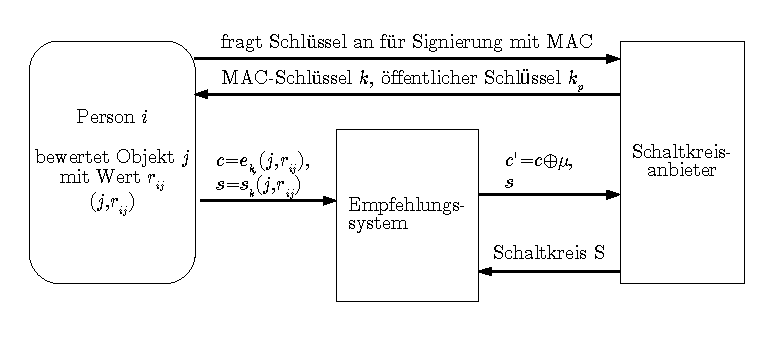
\includegraphics{fig/Matrix}
		\caption{Ablauf zur Erstellung des Schaltkreises der die Matrixfaktorisierung berechnet.}
		\label{fig:Matrix}
	\end{center}
\end{figure}

Die Autoren betrachten zwei Angreifermodelle: Im ersten Fall können das Empfehlungssystem und der Schaltkreisanbieter von einem honest-but-curious Angreifer übernommen werden. Im zweiten Fall wird nur das Empfehlungssystem von einem bösartigen Angreifer übernommen, der sich nicht an das Protokoll hält. In Abbildung \ref{fig:Matrix} wird nur das Design beim stärkeren Angreifermodelle betrachtet:
Damit das Empfehlungssystem die Wertepaare $(j,r_{ij})$ nicht lernt, werden diese von den Personen $i$ unter dem öffentlichen Schlüssel $k_p$ des Schaltkreisanbieters verschlüsselt zu $c=e_{k_s}(j,r_{ij})$. Da das Empfehlungssystem nicht möchte, dass der Schaltkreisanbieter die Wertepaare lernt, werden diese bitweise mit Zufallswerten $\mu$ maskiert zu $c' = c\oplus\mu$. Ein Angreifer könnte Wertepaare verändern oder alle Wertepaare bis auf eines durch Dummywertepaare ersetzen (z.B. alle bewerten das gleiche Modell). Dann gibt der Schaltkreis bei der Matrixfaktorisierung Auskunft welches Objekt eine Person bewertet hat. Damit dies nicht möglich ist, werden Wertepaare vor dem Verschlüsseln von den Personen mit einem MAC-Code signiert, den der erstellte Schaltkreis als zusätzliche Eingabe benötigt. Dazu übergibt der Schaltkreisanbieter der Person einen neuen MAC-Schlüssel je Wertepaar. Der Schaltkreis wird so konstruiert, dass er zu $0$ evaluiert falls der Angreifer Wertepaare verändern sollte.

\textbf{Klassifizierungskriterien:}
\begin{enumerate}
	\item Es wird ein IND-CPA sicheres semihomomorphes Kryptosystem zur XOR Verknüpfung verwendet. Die Autoren entscheiden sich aus Effizienzgründen für die Verwendung von Hash-ElGamal gegenüber dem bekannteren Paillier Kryptosystem. Die Implementierung von Hash-ElGamal ist effizient im Vergleich zu Paillier, dies wird jedoch nicht ausgeführt und auch nicht praktisch verglichen.
	\item Hash-ElGamal wird zur Verschlüsselung und Maskierung durch Addition von Zufallswerten verwendet.
	\item Die Autoren berücksichtigen einen bösartigen Angreifer, der verschlüsselte Wertepaare willkürlich verändern oder komplett ersetzten könnte, indem er selber Wertepaare erzeugt. Dies wird verhindert, indem Wertepaare von den Personen vor dem Verschlüsseln mit einem MAC-code signiert werden.
\end{enumerate}

\section[Efficient and Secure Comparison for On-Line Auctions \cite{damgaard2007efficient}]{\texorpdfstring{Efficient and Secure Comparison for On-Line Auctions\\ \cite{damgaard2007efficient}}{Efficient and Secure Comparison for On-Line Auctions \cite{damgaard2007efficient}}}
\label{dgk}

Damgard et al. motivieren ihre Veröffentlichung damit, dass Vergleiche von verschlüsselten Zahlenwerten vielfältig in privaten verarbeitenden Protokollen benötigt werden. Um Vergleiche höchst performant durchführen zu können, haben sie ein eigenes additiv semihomomorphes Kryptosystem entwickelt (im Folgenden DGK genannt), das IND-CPA sicher ist.

Sie stellen ihr Protokoll für den Fall eines Auktionshauses vor, bei ein aktuelles Höchstgebot $x$ mit einem privaten Gebot $m$ eines Bieters verglichen werden soll. Das aktuelle Höchstgebot $x$ ist öffentlich bekannt. Das Gebot $m$ soll beim Vergleich privat bleiben, damit das Auktionshaus die Preise nicht beliebig erhöhen kann. Denn würde m>x gelten, so wird $x$ nur solange inkrementell erhöht, bis $m$ das Höchstgebot unter allen Bietern ist. Dieses Schema entspricht dem Bieterverfahren bei Ebay.

Für die Kategorisierung werden besondere Designeigenschaften des DGK Kryptosystems untersucht, die das Protokolls ausnutzt: Damit Rechenoperationen bei dem DGK Kryptosystem mit wenig Rechenaufwand erfolgen, soll der Klartextraum $\mathbb{Z}_u$ möglichst klein sein. Sei $l$ die Bitlänge einer zu verschlüsselnden Zahl $m=m_l\ldots m_1$. Dann wählt das Kryptosystem $u$ als die kleinste Primzahl größer als $l+2$. Seien nun $r,r'$ Zufallszahlen\footnote{vgl. mit der Verschlüsselungsfunktion von Okamoto-Uchiyama in \ref{OUK}} und $(n,g,h,u)$ der öffentliche Schlüssel des DGK Kryptosystems. Dann ist eine Eigenschaft des Kryptosystems, dass bei der homomorphen Addition modular reduziert wird bzgl. $u$:

\begin{equation*}
	e_{k_p}(m,r)\cdot e_{k_p}(m',r')\ \text{mod}\ n = e_{k_p}\ (m+m' \text{mod}\,r+r')
\end{equation*}

Da das verwendete Protokoll viele Addition $\text{mod}\ u$ durchführt, soll $u$ möglichst klein sein, aber immer noch genug groß, damit eine modulare Reduktion vermieden wird.

Bei Paillier ist die modulare Reduktion im Klartextraum mit $n=pq$ sehr groß, weil $p,q$ große Primzahlen sind:

\begin{equation*}
	e_{k_p}(m,r)\cdot e_{k_p}(m',r')\ \text{mod}\ n^2 = e_{k_p}(m+m' \text{mod}\ n,r+r')
\end{equation*}

Die Autoren beweisen, dass ihr Kryptosystem IND-CPA sicher ist.

\textbf{Klassifizierungskriterien:}
\begin{enumerate}
	\item Es wurde ein neues Kryptosystem mit kleinen Klartextraum speziell für das Vergleichsprotokoll erstellt um noch schneller private Zahlenvergleiche durchführen zu können als bisherige Umsetzungen. 
	\item Es werden keine weiteren homomorphen Operationen simuliert, die über die Additivität des DGK Kryptosystems hinausgehen.
	\item %Die Autoren beweisen die Sicherheit ihres Vergleichsprotokoll welches das DGK Kryptosystem benutzt unter der Annahme eines honest-but-curious Angreifers. So wird ein unautorisierte Verformbarkeit von Chiffraten durch den Angreifer ausgeschlossen.
	Die Autoren gehen von einem honest-but-curious Angreifer aus.  Eine unautorisierte Verformbarkeit von Chiffraten wird nicht untersucht.
\end{enumerate}

\section{Fingerprinting Protocol for Images Based on Additive Homomorphic Property \cite{kuribayashi2005fingerprinting}}
\label{FPI}
Die Autoren entwerfen ein neues Verfahren, um asymmetrisch Fingerabdrücke in verschlüsselten Bildern zu hinterlegen. Sie benutzen dazu das additiv semihomomorphe Kryptosystem von Okamoto-Uchiyama, um eine möglichst große Verschlüsselungsrate zu erreichen. Bisherige Ansätze um asymmetrisch Wasserzeichen einzubetten benötigten bei einer Datengröße von 1MB bis zu 1GB Kommunikationsdaten. Es wird erwähnt, das der große Klartextraum von Okamoto-Uchiyama eine größere Verschlüsselungsrate ermöglicht.

Um die Einbettung möglichst robust gegenüber Manipulationen zu machen, sollen die Fingerabdrücke im Frequenzraum\footnote{Das \enquote{klassische} RGB Bild ist eine Linearkombination von ortsabhängigen Intensitäten - d.h. Pixeln mit einem Integerwert für die Intensität der Farbe. Man spricht von einer Darstellung im Ortsraum. Eine Fouriertransformation wechselt die Basis unter der das Bild dargestellt wird in den Frequenzraum. Das transformierte Bild wird dargestellt mittels einer Basis aus periodischen Funktionen.} eines Bildes eingebettet werden. Die reellen Zahlen des transformierten Bildes werden zu Integern quantisiert um das Bild verschlüsseln zu können.

Die Einbettung eines Fingerabdrucks erfolgt wie in Abbildung \ref{fig:Finger} veranschaulicht:

\begin{enumerate}
	\item Der Kunde erzeugt einen Fingerabdruck, verschlüsselt ihn mit seinem öffentlichen Schlüssel und sendet den Chiffretext an den Händler. Mit einem Zero-Knowledge-Proof\footnote{Ein Zero-Knowledge-Proof ermöglicht einer Partei A, einer anderen Partei B nachzuweisen das eine Aussage stimmt, ohne mehr als das offenlegen zu müssen (auch: engl. minimal disclosure) \cite{brassard1988minimum}.} wird dem Händler nachgewiesen, dass der Chiffretext tatsächlich einen nutzerspezifischen Fingerabdruck enthält.
	\item Nun verschlüsselt der Händler sein digitales Bild unter dem öffentlichen Schlüssel des Kunden und bettet den Fingerabdruck durch homomorphe Verknüpfung ein.
	\item Der Kunde entschlüsselt das Bild mit dem eingebetteten Fingerabdruck, ohne jedoch in der Lage zu sein diesen zu entfernen.
\end{enumerate}

\begin{figure}[h] 
	\begin{center}
		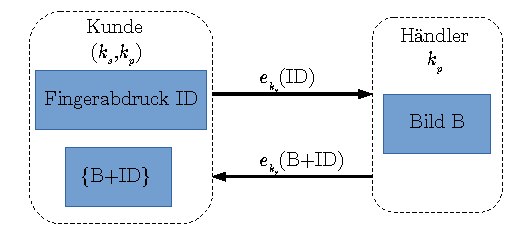
\includegraphics{fig/Finger}
		\caption{Ablauf der Einbettung eines nutzerspezifischen Fingerabdrucks. Die Einbettung erfolgt in dem verschlüsselten digitalen Bild, damit nur der Kunde das Bild mit Fingerabdruck erhalten kann. Würde der Händler Zugriff auf das Bild mit Fingerabdruck haben, könnte er es selber vervielfältigen. }
		\label{fig:Finger}
	\end{center}
\end{figure}

\textbf{Klassifizierungskriterien:}
\begin{enumerate}
	\item Es wird die Asymmetrie des Kryptosystems genutzt um asymmetrische Fingerprints zu erzeugen. Wären die Fingerprints symmetrisch, könnte der Händler den Fingerprint selber einbetten, davon Kopien verbreiten und Kunden hintergehen.\\
	Die Autoren entscheiden sich für das Okamoto-Uchiyama Kryptosystem anstelle von Paillier, weil es weniger Rechenschritte benötigt.
	\item Es werden keine weiteren homomorphen Operationen simuliert, die über die Additivität des Okamoto-Uchiyama Kryptosystems hinausgehen.
	\item Die Autoren erwähnen die Möglichkeit einer unautorisierten Verformbarkeit der Chiffrate, ohne dies bei der Sicherheit ihres Protokolls berücksichtigen zu müssen: Sicherheitsziele in ihrem Verfahren sind, dass der Kunde nicht das Wasserzeichen entfernen kann und der Händler nicht den Fingerabdruck des Kunden entschlüsseln kann. Kunde und Händler weichen nicht vom Protokoll ab (honest-but-curious).
\end{enumerate}

\section{Privacy Preserving Face Recognition \cite{erkin2009privacy} }
\label{PPFR}

Erkin et al. stellen ein Privatsphäre wahrendes Gesichtserkennungssystem vor, bei dem sowohl die Eingabebilder, als auch das Ergebnis ihrer Analyse vom Server nicht im Klartext einsehbar sind. Der Analyse liegt ein Eigenface Algorithmus zugrunde, welcher auf verschlüsselten Bildern arbeitet. Eingesetzt werden die Kryptosysteme Paillier und DGK, welches auch in \ref{dgk} zum Einsatz kommt.

Bei der Schlüsselgenerierung von Paillier wird eine Optimierung aus \cite[p.16]{damgaard2001generalisation} verwendet um den Parameter $g$ des öffentlichen Schlüssels $(n,g)$ zu finden. Sei $n$ wieder $n=pq$ für zwei Primzahlen, dann müsste $g$ nach Paillier \cite{paillier1999public} so gewählt werden, dass $n$ die Ordnung von $g$ teilt. Die Optimierung setzt $g=n+1$ und beschleunigt so die Verschlüsslung.

DGK wird aus Performancegründen zusätzlich zu Paillier eingesetzt. Die Autoren geben dabei wie in \ref{dgk} den kleinen Klartextraum an. Da die Exponenten kleiner sind, ist die Verschlüsselung effizienter.

In den Verschlüsselungsfunktion beider Kryptosysteme werden vom Klartext unabhängige Parameter im Voraus berechnet, um die Verschlüsselung zu beschleunigen. Sei $(n,g)$ der öffentliche Schlüssel unter Paillier und $(n',g',h',u')$ der öffentliche Schlüssel im DGK Kryptosystem. Dann wird der Klartext x mit Zufallszahlen $r,r'$ verschlüsselt zu:

\begin{equation*}
	\text{Paillier: } c = g^x r^n\ \text{mod}\ n^2, \qquad
	\text{DGK: } c = {g'}^x {h'}^{r'}\ \text{mod}\ n'
\end{equation*}

In beiden Kryptosystemen können die Faktoren $r^n$ und ${h'}^{r'}$ bereits im Voraus berechnet werden.

Featurevektoren werden im Algorithmus diskretisiert, indem auf die nächste Ganzzahl gerundet wird, da die Kryptosysteme Ganzzahlen verschlüsseln.

\textbf{Rechenoperationen im Chiffreraum des privaten Gesichtserkennungssystems:}

 Der Eigenface Algorithmus ist trotz der Implementierung auf verschlüsselten Daten vertretbar in der Performance, d.h. der Algorithmus ist in der Lage ein verschlüsseltes Bild von $92\times112$ Pixeln mit 320 Gesichtstemplates der Datenbank in vierzig Sekunden zu vergleichen. Verwendet wird ein Computer mit einem 2.4 GHz AMD Opteron Dualcore Prozessor und 4GB Arbeitsspeicher.
 
 Da eine schnelle Berechnung von komplexen Funktionen auf verschlüsselten Daten nicht selbstverständlich ist, wird die Umsetzung der Rechenoperationen des Eigenface Algorithmus im Folgenden untersucht: Ein in eckige Klammern gesetztes Element bedeutet, dass es mit Alices öffentlichen Schlüssel verschlüsselt ist, die ein Gesicht analysieren möchte. Sie übergibt das verschlüsselte Gesicht und ihren öffentlichen Schlüssel an Bob, der dank homomorpher Kryptographie in der Lage ist den Algorithmus durchzuführen ohne das Gesicht direkt zu sehen.

\begin{figure}[h] 
	\begin{center}
		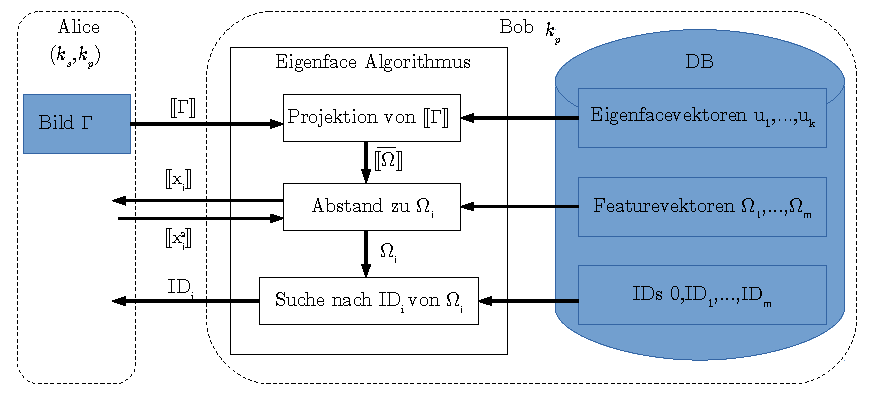
\includegraphics{fig/Faces}
		\caption{Alice möchte die ID (das Gesicht einer Person) wissen. Der Algorithmus extrahiert das Gesichtes aus dem Bild und gleicht es mit der Datenbank von Bob ab. Bob kann den Algorithmus größtenteils alleine ausführen, benötigt jedoch einmal die Hilfe von Alice um ein Zwischenergebnis zu quadrieren.}
		\label{fig:Faces}
	\end{center}
\end{figure}

\begin{itemize} 
\item \textit{Projektion} des verschlüsselten Eingabebildes $\llbracket \Gamma\rrbracket $ auf die Basis von Eigenfacevektoren $u_1,\ldots,u_K$. Die Eigenfacevektoren von Bob sind aus Trainingsdaten entstanden und werden als private Daten betrachtet, die Alice nicht lernen darf. Bei der Projektion wird mit der gleichen Technik wie in \ref{ML} ein Skalarprodukt durch Potenzieren berechnet. Das Ergebnis ist ein verschlüsselter Featurevektor des Eingabebildes  $\llbracket\overline\Omega\rrbracket$, welcher nun mit Featurevektoren der Datenbank verglichen werden kann um das Gesicht zuzuordnen.
\item \textit{Abstand} $D$ von Featurevektoren $\{\Omega_1,\ldots,\Omega_M\}$ der Datenbank von Bob zum Featurevektor des Eingabebildes $\llbracket\overline\Omega\rrbracket$. Da man nur an der relativen Ordnung der Abstände interessiert ist, genügt der Vergleich der quadierten Abstände:
\begin{equation}
\label{Aufteilung}
\begin{aligned}
D(\Omega,\overline\Omega)
&=
\|\Omega-\overline\Omega\|^2=(\omega_1-\overline\omega_1)^2+\ldots+(\omega_K-\overline\omega_K)^2\\
&=
\underbrace{\sum_{i=1}^{K}\omega_{i}^2}_{S_1}+
\underbrace{\sum_{i=1}^{K}(-2\omega_i\overline\omega_i)}_{S_2}+
\underbrace{\sum_{i=1}^{K}\overline\omega_{i}^2}_{S_3}
\end{aligned}
\end{equation}

Nun werden die drei Summenblöcke getrennt zur Berechnung des verschlüsselten Abstands $\llbracket D(\Omega,\overline\Omega)\rrbracket$ verwendet:
Da Bob den Server betreibt, kennt er die Komponenten $\omega_i$ der Featurevektoren in der Datenbank und kann $S_1$ direkt im Klartext berechnen und \textit{anschließend} mit Alices öffentlichen Schlüssel verschlüsseln. Da er die Komponenten $\overline\omega_i$ des Featurevektor vom Eingabebild nur verschlüsselt vorliegen hat, muss er $S_2$ analog wie beim Skalarprodukt in \ref{ML} durch potenzieren berechnen. Letztendlich kann Bob $S_3$ nur in Kooperation mit Alice berechnen, da ihm bei beide Faktoren des Produkts unbekannt sind. Dazu maskiert er die Komponenten des Featurevektors mit gleichverteilten Zufallswerten $r_i$, um sie vor Alice zu verschleiern:
\begin{equation*}
\llbracket x_i \rrbracket = \llbracket\overline\omega_i+r_i\rrbracket
\end{equation*}
Diese maskierten Komponenten sendet er an Alice, welche diese mit ihrem privaten Schlüssel entschlüsselt und quadriert, das Ergebnis $\llbracket x_{i}^2\rrbracket$ wieder verschlüsselt und dann an Bob zurücksendet. Bob berechnet dann den i-ten Summand von  $S_3$ durch:

\begin{equation*}
\llbracket x_i^2 \rrbracket\cdot\llbracket\overline\omega_i\rrbracket^{(-2r_i)}\cdot\llbracket-r_i^2\rrbracket =
\llbracket (\overline\omega_i+r_i)^2-2r_i\overline\omega_i - r_i^2 \rrbracket = \llbracket\overline\omega_i^2 \rrbracket 
\end{equation*}

Die Aufsummierung der $\llbracket\overline\omega_i^2\rrbracket$ und sowie von $\llbracket S_1\rrbracket,\llbracket S_2\rrbracket,\llbracket S_3\rrbracket$ kann Bob nun im Chiffreraum homomorph durch Multiplikation der Chiffretexte durchführen und erhält so $\llbracket D(\Omega,\overline\Omega)\rrbracket$ (vgl. homomorphe Addition bei Okamoto-Uchiyama \ref{OUK}).

\item \textit{Vergleich} zweier verschlüsselter Zahlen im DGK Kryptosystem. Hier setzten die Autoren das Protokoll von \ref{dgk} ein.
\end{itemize}

\textbf{Klassifizierungskriterien:}
\begin{enumerate}
	\item Diese Studie zeigt, dass komplexe Funktionen auf verschlüsselten Daten berechnet werden können ohne auf ein vollhomomorphes Kryptosystem angewiesen zu sein. Es wird eine Optimierung bei der Schlüsselgenerierung verwendet, die spezifisch für Paillier ist. Optimierungen bei der Verschlüsselung durch Vorberechnungen lassen sich auch auf andere semihomomorphe Kryptosysteme übertragen. Um den Eigenface Algorithmus zu beschleunigen, wird das Kryptosystem DGK für den Vergleich von Zahlen eingesetzt.
	\item Es wird eine Projektion mit Skalarprodukten und ein quadratischer Abstand zwischen zwei Zahlen berechnet. Diese Berechnungen sind allerdings nur möglich, weil eine der Zahlen unverschlüsselt in die Berechnung eingeht. Weiter wird bei beim quadratischen Abstand auf das Wurzelziehen verzichtet, da man nur an einem relativen Vergleich der Ergebnisse interessiert ist.
	\item Bei der Skalarproduktberechnung wäre es Alice möglich durch Erstellen eines Vektors, bestehend aus neutralen Elementen in allen Komponenten, Bobs privaten Vektor $u_i$ zu lesen. Aber im Ablauf des Eigenface Algorithmus erhält Alice das Ergebnis dieser Rechenoperation nicht zurück. Um Zwischenergebnisse des Algorithmus anzugreifen, müssen Alice und Bob vom Ablauf des Eigenface Algorithmus abweichen, was jedoch ausgeschlossen wird, da von einem honest-but-curious Angreifer ausgegangen wird.
\end{enumerate}

\section{Private predictive analysis on encrypted medical data \cite{bos2014private}}
\label{PAMD}

Joppe W. Bos et. al stellen ein Verfahren vor, in dem ein statistisches Vorhersagemodell auf komplett verschlüsselten Daten arbeitet. Der Client verschlüsselt die medizinischen Daten mit seinem öffentlichen Schlüssel und übergibt diese dem Server. Dort wird ohne Einsatz des privaten Schlüssels und ohne weitere Interaktion mit dem Clienten eine Analyse auf den verschlüsselten Daten durchgeführt. Der Client erhält im Anschluss das verschlüsselte Ergebnis.

Der Server führt eine logistische Regression auf den homomorph verschlüsselten Daten durch, um die Wahrscheinlichkeit einer Herzkreislauferkrankung zu vorherzusagen. Zum Einsatz kommt ein beschränkt (hier: leveled) vollhomomorphes Kryptosystem \cite{bos2013improved} mit Optimierungen aus \cite{brakerski2012fully} (im Folgenden BLLN genannt). Das BLLN Kryptosystem ist IND-CPA sicher. Die Autoren haben sich für dieses Kryptosystem entschieden, da die Chiffretexte bei homomorphen Multiplikationen nicht expandieren\footnote{Es wird weniger Speicherplatz benötigt, dafür ist die Rechenzeit in der Ausführung größer. Wie in \ref{VHKK} erwähnt ist die Expansion der Chiffretext ein Problem bei Vollhomomorphen Kryptosystemen.}, dafür ist gegenüber dem Kryptosystem von Brakerski el al. (\ref{ML}) die Multiplikation langsamer.
 
In dem Vorhersagemodell mit logistischer Regression wird folgende Prädiktionsformel berechnet:
\begin{equation*}
P(x) = \frac{e^x}{e^x-1}.
\end{equation*}
Die Eingabe x ist eine Linearkombination von patientspezifischen Parametern, die mit  Regressionskoeffizienten gewichtet sind. Somit ist x homomorph berechenbar. Die Prädiktionsformel wird homomorph berechenbar durch Annäherung mit einer Taylorreihe siebten Grades.

Eine Besonderheit des BLLN Kryptosystems ist die Struktur vom Klartext- und Chiffreraum. Sowohl Klartext als auch Chiffretexte repräsentieren Polynome mit ganzzahligen Koeffizienten der Art  $\sum_{i=0}^{n-1} a_i X^i, a_i\in\mathbb{Z}$. Die Elemente sind aus dem Polynomring  $R=\mathbb{Z}/(X^n+1)$. Operationen im Chiffreraum entsprechen der Addition und Multiplikation von Polynomen mod $X^n+1$. 

\textbf{Anmerkungen:}
Die Autoren sprechen nicht ausdrücklich von einem honest-but-curious Angreifer. Bei der Sicherheit der Implementierung werden nur kryptografische Angreifer betrachtet. Man geht jedoch davon aus, dass Client und Server nicht vom Protokoll abweichen. Dies entspricht dem honest-but-curious Angreifermodell.

\textbf{Klassifizierungskriterien:}
\begin{enumerate}
	\item Es wird das beschränkt vollhomomorphe Kryptosystem BLLN eingesetzt um Polynome zu berechnen. BLLN wird gegen über BGV präferiert, da Chiffretext bei Multiplikation nicht größer werden. 
	\item Es wird eine Exponentialfunktion linearisiert, um das Taylorpolynom mit BLLN berechenbar zu machen.
	\item Das Kryptosystem ist IND-CPA sicher. Die Autoren gehen nicht auf eine unautorisierte Verformbarkeit der Chiffretexte ein. Der Cloudservice interagiert nicht mehr mit dem Clienten nach Erhalt der verschlüsselten Daten. Um eine unautorisierte Verformbarkeit der Chiffretexte auszunutzen, müsste man von einem Angreifer ausgehen, der neben dem Cloudservice auch den Clienten kontrolliert. Aber in diesem Fall hätte der Angreifer Zugriff auf den privaten Schlüssel und alle hinterlegten Daten. 
\end{enumerate}  

\section{Klassifizierung}
\label{klassSum}

Im Folgenden sind die Ergebnisse der Untersuchungen aus diesem Kapitel zusammengefasst.

\subsection{Anwendungsfälle der Kryptosysteme}
\label{EdK}

Die erste Tabelle fasst die Anwendungsfälle der Kryptosysteme zusammen und ist daher nach den Veröffentlichungen sortiert. Neben dem verwendeten Kryptosystem wird angegeben auf welche Kryptobibliothek zurückgegriffen wurde, bzw. ob sich die Autoren sich für eine eigene Implementierung entschieden haben. Da asymmetrische homomorphe Kryptosysteme in Protokollen mit mehreren Parteien eingesetzt werden, wird in der Spalte $\rightarrow\textit{Angreifer}$ angegeben, ob ein Angreifermodell nach Abschnitt \ref{hbc} betrachtet wird. In der Spalte  $\rightarrow\textit{Integritätsprüfung der Chiffretexte}$ wird angegeben, ob die Autoren die Integrität der Chiffretexte prüfen. Die Spalte $\rightarrow\textit{Chiffretextwechsel}$ gibt an, ob zwischen mehreren Kryptosystemen in einem Anwendungsfall gewechselt wird. 

\textbf{Anmerkungen zur ersten Tabelle:}
In den Veröffentlichungen \ref{FPI} und \ref{PAMD} interagieren die Parteien nur einmal. Im honest-but-curious Angreifermodell bekommt der Angreifer nicht wieder Zugriff auf den verformten Chiffretext, ohne vom Protokoll abweichen zu müssen. Die einzige andere Möglichkeit für den Angreifer, um an den Chiffretext zu kommen, ist, wenn er beide Parteien kontrolliert. Denn würde der Angreifer beide Parteien kontrollieren, wäre er im Besitz des privaten Schlüssels und könnte alle Chiffretexte entschlüsseln. Bei einem honest-but-curious Angreifermodell geht man jedoch davon aus, dass der Angreifer höchstens $n/2$ der Parteien kontrolliert (hier: 1) (Siehe dazu die Definition in Abschnitt \ref{hbc}).  In vielen der vorgestellten Anwendungsfälle ist eine unautorisierte Verformbarkeit der Chiffretexte damit \textit{nicht ausnutzbar}.

\noindent
\definecolor{light-gray}{gray}{0.95}
\rowcolors{1}{white}{light-gray}
\begin{tabu}{ | l | p{4.5cm} |  p{1.6cm} |  p{4.3cm} |}
	\hline
	Veröffentlichung & Kryptosystem\newline(Implementierung) & Angreifer & Integritätsprüfung der\newline Chiffretexte \\ \hline  \tabucline[1pt]{-}
	
	\ref{autocrypt}, \cite{tople2013autocrypt} 
	& ElGamal (libcrypt \cite{libcrypt:online}),
	  \newline Paillier (CryptDB \cite{popa2011cryptdb})
	& Bösartig\footnote{Das transformierte Programm läuft auf einem nicht vertrauenswürdigen Webserver. Der Angreifer kann die Eingaben des Programms ersetzen. Dies entspricht dem Modell eines bösartigen Angreifers.}
	& Nein, ausdrücklich nicht berücksichtigt \\ \hline
	
	\ref{ML}, \cite{bost2015machine} 
	& Goldwasser-Micali, Paillier\newline (jeweils eigene Implementierung \cite{ciphermed:online} in C++ mit GMP \cite{gmp:online} und NTL \cite{nlt:online}),\newline BGV (HElib \cite{HElib:online}\cite{halevi2013design})
	& HBC 
	& Nein\\ \hline
	
	\ref{PPMF}, \cite{nikolaenko2013privacy}
	& Hash-ElGamal\newline (eigene Implementierung\footnote{Die Autoren haben die Algorithmen des Kryptosystems vermutlich selber implementiert. Sie machen hierzu jedoch keine Aussage. % Der Quellcode ist nicht veröffentlicht.
		\label{note2}})
	& Bösartig
	& Signierung mit MAC-Code  \\ \hline
	
	\ref{dgk}, \cite{damgaard2007efficient}
	& DGK\newline (eigene Implementierung in Java 1.5 unter Verwendung der Klasse BigInteger)
	& HBC
	& Nein \\ \hline
	
	\ref{FPI}, \cite{kuribayashi2005fingerprinting}
	& Okamoto-Uchiyama\newline(eigene Implementierung %\footnote{Die Autoren haben die Algorithmen des Kryptosystems selber implementiert. Der Quellcode ist nicht veröffentlicht.}
	)
	& HBC
	& unautorisierte Verformbarkeit nicht ausnutzbar: ein verformter Chiffretext wird im Protokoll nicht mehr zurück erhalten und der Angreifer kontrolliert höchstens eine Partei \\ \hline
	
	\ref{PPFR}, \cite{erkin2009privacy} 
	& Paillier, DGK\newline (jeweils eigene Implementierung mit kryptografischen Optimierungen aus \cite{damgaard2001generalisation} in C++ mit GMP \cite{gmp:online})
	& HBC
	& Nicht ausnutzbar im HBC Modell, da nicht vom Protokoll abgewichen wird. \\ \hline
	
	\ref{PAMD}, \cite{bos2014private}	
	& BLLN\newline (eigene Implementierung mit kryptografischen Optimierungen aus \cite{brakerski2012fully})
	& HBC
	&  unautorisierte Verformbarkeit nicht ausnutzbar: ein verformter Chiffretext wird im Protokoll nicht mehr zurück erhalten und der Angreifer kontrolliert höchstens eine Partei\\ \hline
\end{tabu}

\noindent
\begin{tabu}{ | l | p{4.9cm} |p{6cm}|}
	\hline
	Veröffentlichung & Chiffretextwechsel & Grund für Chiffretextwechsel\\ \hline  \tabucline[1pt]{-}
	
	\ref{autocrypt}, \cite{tople2013autocrypt} 
	& ElGamal $\leftrightarrow$ Paillier
	& Durchführung von Addition und Multiplikation mit gleicher Variable \\ \hline

	\ref{ML}, \cite{bost2015machine}
	& Goldwasser-Micali $\rightarrow$ BGV
	\newline  Goldwasser-Micali  $\rightarrow$ Paillier 
	&  Evaluierung von Polynomen,
	\newline Weiterrechnen unter Paillier\\ \hline	
	
	\ref{PPMF}, \cite{nikolaenko2013privacy}
	& -
	& - \\ \hline
	
	\ref{dgk}, \cite{damgaard2007efficient} 
	& -
	& -\\ \hline	
	
	\ref{FPI}, \cite{kuribayashi2005fingerprinting}
	& - 
	& - \\ \hline
	
	\ref{PPFR}, \cite{erkin2009privacy}  
	& Paillier $\rightarrow$ DGK
	& schnellere Vergleiche\\ \hline
	
	\ref{PAMD}, \cite{bos2014private}	 
	& -
	& - \\ \hline
\end{tabu}

\subsection{Auswahlkriterien und Eigenschaften der Kryptosysteme}

Die zweite Tabelle fasst Auswahlkriterien der homomorphen Kryptosysteme zusammen, die in den Veröffentlichungen genannt wurden. Dazu werden grundlegende Eigenschaften der Kryptosysteme aufgelistet.
% Die Tabelle wird um weitere Kryptosysteme ergänzt die in der Recherche gefunden wurden.
% Einzelne Eigenschaften wie die Chiffretextexpansionsrate $\rightarrow\textit{Expansion}$ oder die Sicherheit gegenüber Angreifermodelle der Kryptoanalyse aus Abschnitt \ref{angreifermodelle} $\rightarrow\textit{Sicherheit}$ wird durch weitere Quellen belegt.
%In der Kommentarspalte sind Beziehungen zwischen den Kryptosystem aufgelistet.

$\rightarrow\textit{LVHE}$ steht für leveled vollhomomorphes Kryptosystem, $\rightarrow\textit{SH}$ steht für semihomomorphes Kryptosystem, $\rightarrow\textit{OP}$ steht bei semihomomorphen Kryptosystemen für realisierte Rechenoperationen mit diesem Kryptosystem, $\rightarrow\textit{konst-*}$ steht für Konstantenmultiplikation durch Potenzierung.

\noindent
%\rowcolors{1}{white}{light-gray}
\begin{tabu}{ | p{3cm} |p{6cm} | l | p{1.2cm} | l |}
	\hline
	Kryptosystem & Auswahlkriterien & Typ & OP  & Sicherheit  \\ \hline \tabucline[1pt]{-}
	
	BGV \cite{Brakerski2012LeveledFH}
	& Evaluation von Polynomen  
	& LVHE
	& LVHE
	& IND-CPA\\ \hline
	
	BLLN \cite{bos2013improved}
	& Evaluation von Polynomen, keine Chiffretextexpansion bei Multiplikation, jedoch langsamer als BGV
	& LVHE
	& LVHE
	& IND-CPA\\ \hline
	
	DGK \cite{damgaard2007efficient}
	& Speziell entwickelt für schnelle Vergleiche, kleiner Klartextraum
	& SH
	& +
	& IND-CPA  \\ \hline
	
	ElGamal  \cite{yi2014homomorphic}
	& Homomorphe Multiplikation
	& SH 
	& * 
	& IND-CCA1 \\ \hline
	
	Goldwasser-Micali \cite{goldwasser1984probabilistic}
	& Vergleiche nach Protokoll \cite{veugen2011comparing}
	& SH
	& XOR %Buch
	& IND-CPA\\ \hline
	
	Hash-ElGamal \cite{nikolaenko2013privacy}
	& Effizienter als additive SH Kryptosysteme um Chiffretexte zu maskieren
	& SH 
	& XOR
	& IND-CPA \\ \hline
		
	Okamoto-Uchiyama \cite{okamoto1998new}
	& Einfachere Implementierung als bei Paillier, da weniger Rechenschritte
	& SH
	& +, \newline konst-*
	& IND-CPA \\ \hline
	
	Paillier \cite{paillier1999public}
	& Großer Klartextraum ermöglicht Verschlüsselung von Fließkommazahlen durch Multiplikation mit großen Exponenten,
	\newline XOR durch Verschlüsselung der Integerbits in \ref{autocrypt},
	\newline privates Skalarprodukt,
	\newline Vergleiche nach Protokoll \cite{veugen2011comparing}
	& SH 
	& +,  \newline XOR, \newline $\langle\cdot,\cdot\rangle$, \newline konst-*
	& IND-CPA \\ \hline
	
\end{tabu}

Damit lassen sich folgende Klassen nach Einsatzszenarien identifizieren:
\begin{enumerate}
	\item \textit{Evaluation von Polynomen} durch leveled vollhomomorphe Kryptosysteme: BGB, BLLN. Obwohl sich Polynome durch Kombinationen von semihomomorphen Kryptosystemen berechnen lassen, wurden leveled vollhomomorphe Kryptosysteme eingesetzt.
	\item  \textit{Vergleiche} durch spezialisierte Kryptosysteme: DGK. Das Kryptosystem ist für eine schnelle Ausführung optimiert.
	\item \textit{Flexibel einsetzbare} Kryptosysteme: Paillier, Okamoto-Uchiyama. Beide Kryptosysteme verschlüsseln Ganzzahlen, können aber auch auf der Bitdarstellung der Ganzzahlen verwendet werden, um Bitoperationen wie XOR im Chiffreraum zu ermöglichen. Beide Kryptosysteme ermöglichen eine Konstantenmultiplikationen durch Potenzierung, wodurch komplexere Operatoren berechnet werden können (Skalarprodukt, quadratischer Abstand).
\end{enumerate}
Weiter gibt es Kryptosysteme, in denen die Verschlüsselungsfunktion teilweise im Voraus berechenbar ist. Da diese Klasse jedoch kein Einsatzszenario festlegt, wird diese Klasse gesondert angegeben: 
\begin{enumerate}
	 \item[\color{NavyBlue}(4.)] \textit{Vorausberechenbare} Kryptosysteme: Paillier, Okamoto-Uchiyama\footnote{In Abschnitt \ref{OUK} kann der Faktor $h^r$ vorausberechnet werden.}, DGK. Faktoren der Verschlüsselungsfunktion, die nicht vom Klartext abhängen, können im Voraus werden. Dazu müssen zu Zufallszahlen erzeugt werden.
\end{enumerate}







%Alles Kryptosysteme arbeiten auf Untergruppen Z_n, d.h. sie verschlüsseln Integer.


%Auf Vergleich der Performanz der Kryptosysteme ist anhand vorliegender Studien alleine nicht möglich